\documentclass{article}
\usepackage{tikz,tkz-graph}
\begin{document}
\definecolor{maize}{HTML}{FFCB05}
\definecolor{theblue}{HTML}{00274C}
\begin{figure}
\SetVertexNormal[Shape      = circle,
                 FillColor  = maize,
                 LineWidth  = 2pt]
\SetUpEdge[lw         = 1.5pt,
           color      = black,
           labelcolor = white,
           labeltext  = red,
           labelstyle = {draw,text=theblue}]
\tikzset{EdgeStyle/.style={->}}
\tikzset{VertexStyle/.style = {text = theblue, shape=circle, fill=maize, line width=2pt, draw = theblue}}
\begin{center}
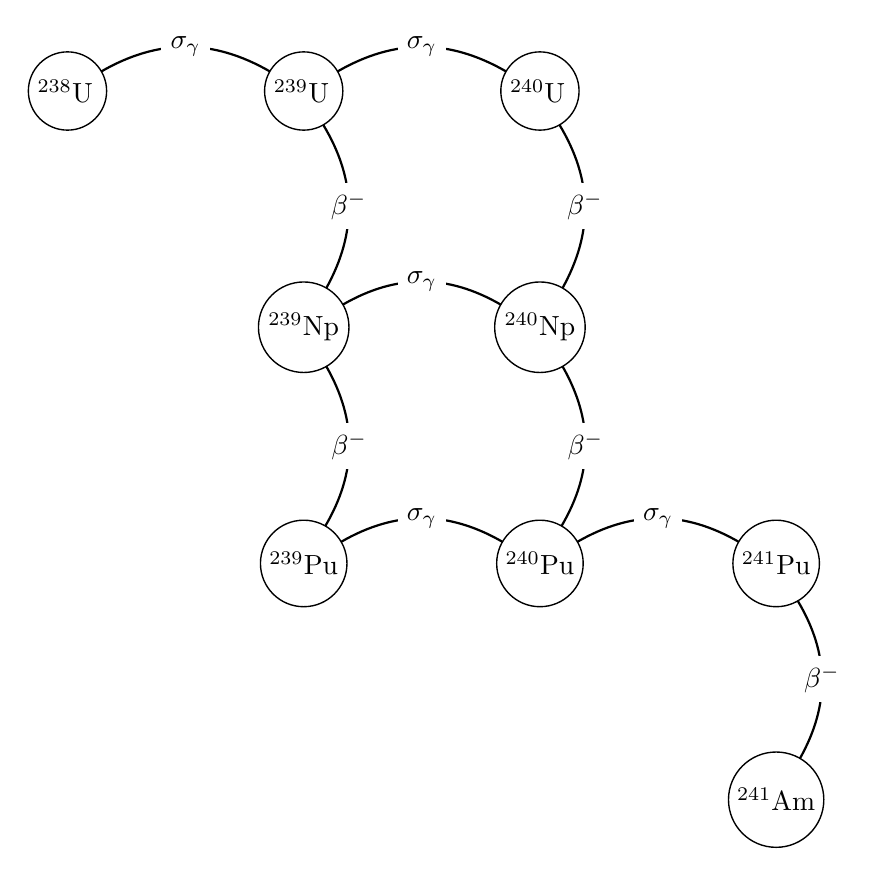
\begin{tikzpicture}[scale=1]
   \Vertex[Math,L=^{238}\mathrm{U\,},x=0 ,y=7]{U238}
   \Vertex[Math,L=^{239}\mathrm{U\,},x=3 ,y=7]{U239}
   \Vertex[Math,L=^{240}\mathrm{U\,},x=6 ,y=7]{U240}
   \Vertex[Math,L=^{239}\mathrm{Np},x=3 ,y=4]{Np239}
   \Vertex[Math,L=^{240}\mathrm{Np},x=6 ,y=4]{Np240}
   \Vertex[Math,L=^{239}\mathrm{Pu},x=3 ,y=1]{Pu239}
   \Vertex[Math,L=^{240}\mathrm{Pu},x=6 ,y=1]{Pu240}
   \Vertex[Math,L=^{241}\mathrm{Pu},x=9 ,y=1]{Pu241}
   \Vertex[Math,L=^{241}\mathrm{Am},x=9 ,y=-2]{Am241}
   \tikzset{EdgeStyle/.append style = {bend left}}
   \Edge[label = $\sigma_\gamma$](U238)(U239)
   \Edge[label = $\sigma_\gamma$](U239)(U240)
   \Edge[label = $\beta^-$](U239)(Np239)
   \Edge[label = $\beta^-$](U240)(Np240)
   \Edge[label = $\sigma_\gamma$](Np239)(Np240)
   \Edge[label = $\beta^-$](Np239)(Pu239)
   \Edge[label = $\beta^-$](Np240)(Pu240)
   \Edge[label = $\beta^-$](Pu241)(Am241)
   \Edge[label = $\sigma_\gamma$](Pu239)(Pu240)
   \Edge[label = $\sigma_\gamma$](Pu240)(Pu241)
\end{tikzpicture}
\end{center}
\caption{A transmutation network for $^{238}$U.}\label{fig:full_u238}
\end{figure}

\end{document}